%=== Chapter One ===
\chapter{Introduction}

\ifpdf
    \graphicspath{{Chapter1/Chapter1Figs/PNG/}{Chapter1/Chapter1/PDF/}{Chapter1/Chapter1Figs/}}
\else
    \graphicspath{{Chapter1/Chapter1Figs/EPS/}{Chapter1/Chapter1/}}
\fi

\section{Introduction}

Defining and distinguishing phases of matter has been a continuing effort by physicists for many years. 

\section{1D Topological Superconductor}

In order to illustrate the essential elements of a topological condensed matter system, we now present a construction and analysis of the simplest superconducting lattice model, the Kitaev wire \cite{Kitaev01}. 

\subsection{Dirac fermions}

Given $N\in\mathbb{N}^{+}$ Dirac fermions, hereby denoted simply as fermions, they can be represented by a set of second quantised fermionic field operators $\{a_{j}\}$ and their conjugate partners $\{a_{j}^{\da}\}$, where $j=1,...,N$. They obey the following commutation relations
\begin{align}
    &\{a_{i},a_{j}^{\da}\}=\delta_{ij} &\{a_{i}^{(\da)},a_{j}^{(\da)}\}=0
\end{align}
    
\noi where $\delta_{ij}$ Kronercker delta function. These operators act on a tensor product of Fock states. A general state of the fermionic system, $\ket{\psi}$ can be written as
\begin{equation}
    \ket{\psi}=\sum_{n_{i}=0,1}\Bigg(\alpha_{n_{1},...,n_{N}}\bigotimes_{i=1}^{N}\ket{n_{i}}\Bigg),
\end{equation}

\noi where $\alpha_{n_{1},...,n_{N}}\in\mathbb{C}$ and
\begin{equation}
    \bigotimes_{j=1}^{N}\ket{n_{j}}=\Bigg(\bigotimes_{j=1}^{N}\big(a^{\da}_{j}\big)^{n_{j}}\Bigg)\Bigg(\bigotimes_{j=1}^{N}\ket{0}\Bigg).
\end{equation}

\subsection{Real space tight-binding model}

\begin{figure}
    \begin{center}
        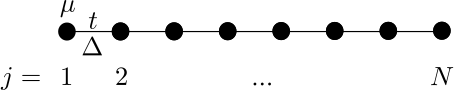
\includegraphics[scale=0.65]{Chapter1/Chapter1Figs/PDF/1DSUPCHAIN}
    \end{center}
    \caption{A schematic representation of the Kitaev 1D wire. A set of $N$ sites denoted by the black dots and indexed by $j=1,..,N$ are connected by black lines. To each site we associate a fermion $a_{j}$ to which we associate a chemical potential $\mu\in\mathbb{R}$. We allow for fermions to tunnel to adjacent sites with amplitude $t\in\mathbb{R}$ and pair with adjacent fermions with amplitude $\Delta\in\mathbb{R}$ }
    \label{fig:1DSUPCHAIN}
\end{figure}

We take a chain of $N$ sites indexed by $j=1,...,N$ and to each site we associate a fermion $a_{j}$. To each fermion we associate the same chemical potential $\mu$ and we allow for nearest neighbour tunnelling and pairing with amplitudes $t$ and $\Delta$ respectively, with $\mu,t,\Delta\in\mathbb{R}$. This arrangement is shown in fig. \ref{fig:1DSUPCHAIN}. With this information we can write down a tight binding Hamiltonian
\begin{equation}\label{eqn:KITHAM}
    H = \sum_{j=1}^{N}\Big(\mu a_{j}^{\da}a_{j}-\frac{1}{2} + t a_{j}^{\da}a_{j+1} + \Delta a_{j}a_{j+1}\Big) + h.c.,
\end{equation}

\noi where $h.c.$ denotes the Hermitian conjugate. We have chosen periodic boundary conditions such that $N+1$ is $1$.

\subsection{Momentum space and the Fourier tansform}

Because \eqref{eqn:KITHAM} is translationally invariant and has preiodic boundary conditions, we can transform it into momentum space via the Fourier transform. The transformation is defined as
\begin{align}
    &a_{j}=\sum_{p}e^{ipj}a_{p} &a_{j}^{\da}=\sum_{p}e^{-ipj}a^{\da}_{p},
\end{align}

\noi where $p\in[-\pi,\pi)$, also called the Brillouin zone (BZ). The transformed Hamiltonian is written as
\begin{equation}
    H = \sum_{p} \big(\mu + t\cos(p)\big)\Big(a_{p}^{\da}a_{p} -a_{-p}a_{-p}^{\da}\Big) + i\Delta\sin(p)\Big(a_{p}a_{-p} - a_{-p}^{\da}a_{p}^{\da}\Big).
\end{equation}

We can now write the Hamiltonian in Bogoliubov-de Gennes form 
\begin{equation}
    H = \sum_{p}\bs{\psi}_{p}^{\da}h(\bs{\lambda},p)\bs{\psi}_{p},
\end{equation}

\noi where $\bs{\psi}_{p}=\bpm a_{p} & a_{-p}^{\da}  \epm ^{\text{T}}$, $\bs{\lambda}=\bpm \mu & \Delta & t \epm$, and $h(p)$ is a $2\times2$ Hermitian matrix given by
\begin{equation}\label{eqn:KITKERN}
    h(p) = \bpm \epsilon(p) & \Xi(p) \\ \Xi^{*}(p) & -\epsilon(p) \epm
\end{equation}

\noi where $\epsilon(\mu,t,p)=\mu+t\cos(p)$ and $\Xi(\Delta,p)=i\Delta\sin(p)$. We shall call $h(\bs{\lambda},p)$ the \emph{kernel Hamiltonian}. From the kernal Hamiltonian we can extract many useful quantities such as the energy spectrum and the model's topological invariant, the winding number.

\subsection{Symmetries}

Free fermionic models can be classified by the symmetries of the kernel Hamiltonian \cite{Ryu10,Wen12,Schnyder08}. The presence (or not) of time-reversal (TR), particle-hole (PH) and sublattice (S) symmetries determines which of 10 classes a given Hamiltonian is in. More shall be said of the so called 10-fold way later in this document. The model as it stands obeys both TR and PH symmetries and by implication S symmetry.  

\subsection{Energy Spectrum and ground state}

The model supports a pair of eigenvalues and eigenvectors, $E^{\pm}(\bs{\lambda},p)$ and $\ket{\psi_{\pm}(\bs{\lambda},p)}$. As the model is PH symmetric the spectrum will be symmetric about zero energy. This is confirmed when we look at the analytic expression for the eigenvalues of \eqref{eqn:KITKERN}, 
\begin{equation}
    E^{\pm}(\bs{\lambda},p)=\pm\sqrt{|\epsilon(\mu,t,p)|^{2} + |\Xi(\Delta,p)|^{2}}.
\end{equation}

\begin{figure}
    \begin{center}
        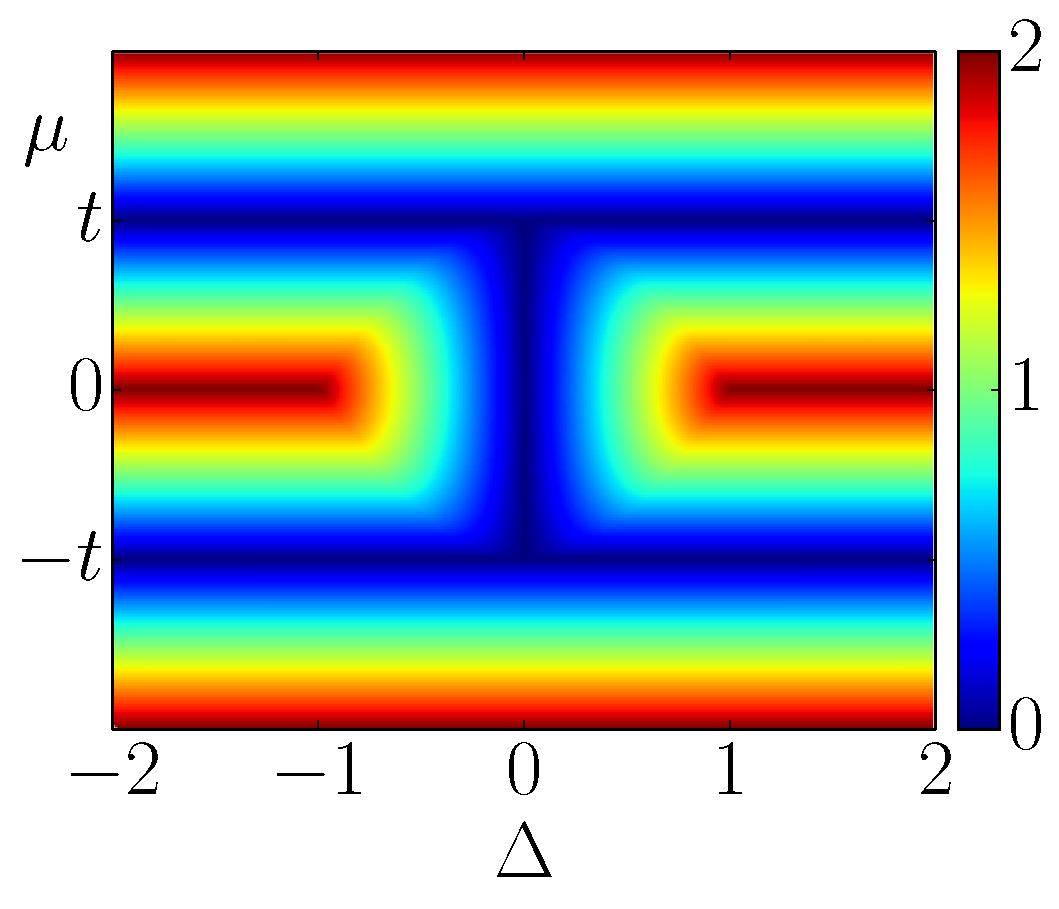
\includegraphics[scale=0.4]{Chapter1/Chapter1Figs/PDF/kitwind.pdf}
        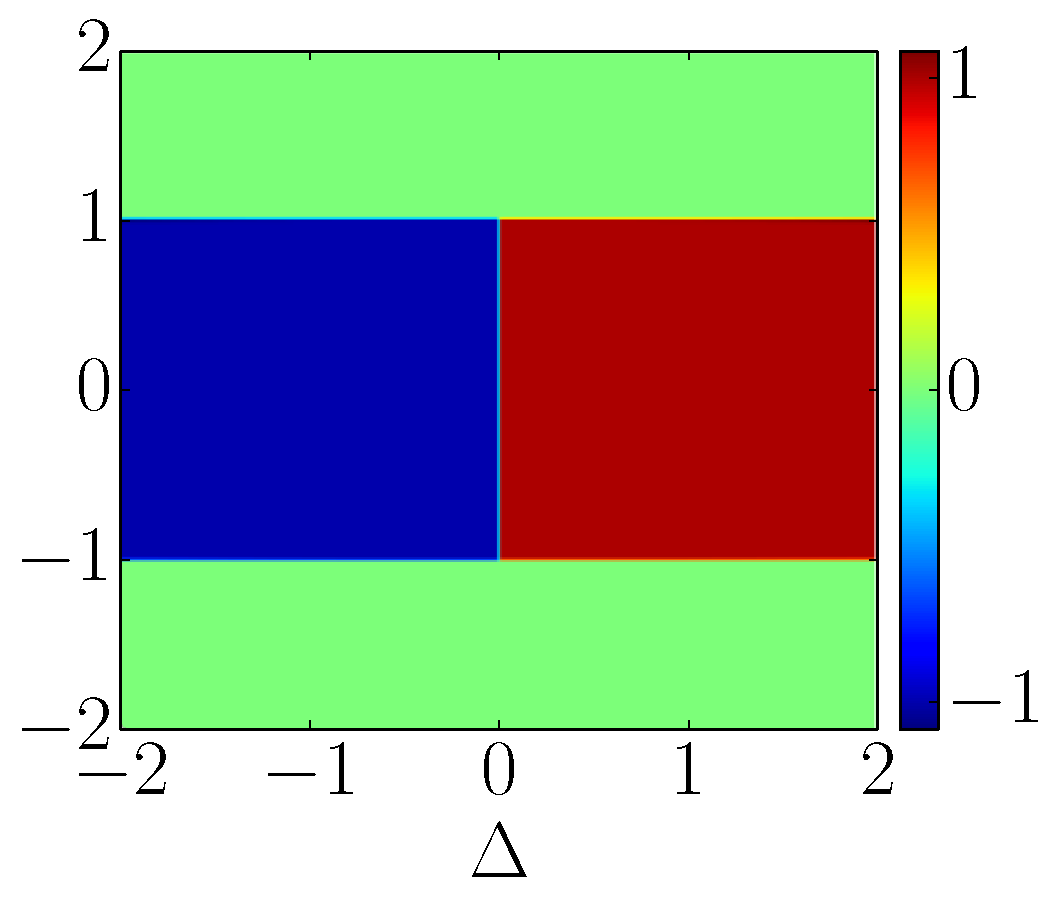
\includegraphics[scale=0.4]{Chapter1/Chapter1Figs/PDF/kitgap.pdf}
    \end{center}
    \caption{(Left) The energy gap, $\Delta E$ of the Kitaev wire as a function of the chemical potential, $\mu$, and the superconducting order parameter $\Delta$ with $t=1$. The data was obtained via exact diagonalisation of \eqref{eqn:KITKERN}. (Right) The winding number, $\nuone$, of the Kitaev wire. Each gapped phase is separated by a gappless line as depicted in the diagram of the gap on the left. The data was obtained via numerical evaluation of \eqref{eqn:1DWIND}. }
    \label{fig:kitspec}
\end{figure}

\noi We define the \emph{energy gap}, denoted $\Delta E(\bs{\lambda})$, as 
\begin{equation}
    \Delta E(\bs{\lambda})=2\cdot\text{min}_{p}|E^{+}(\bs{\lambda},p)|.
\end{equation}

\noi In fig. \ref{fig:kitspec} (left) we plot $\Delta E(\bs{\lambda})$ as a function of $\mu$ and $\Delta$ and for $t=1$. The diagram is separated into four regions where $\Delta E(\bs{\lambda})\neq0$ which are separated by lines where $\Delta E(\bs{\lambda})=0$.\\

We take the system to be at half filling. This means that all of the negative energy states are occupied and the ground state is state associated with $E^{-}(p)$, $\ket{\psi_{gs}(p)}=\ket{\psi_{-}(p)}$. 

\subsection{Winding number}

The topological phase of the system is determined by the winding number, $\nuone$. In order to define $\nuone$ we must first define a unit vector $\bs{\hat{s}}(p)$ which parametrises the kernel Hamiltonian
\begin{equation}
    h(\bs{\lambda},p) = \bs{s}(\bs{\lambda},p)\cdot\bs{\sigma}=|\bs{s}(\bs{\lambda},p)|\bs{\hat{s}}(\bs{\lambda},p)\cdot\bs{\sigma}
\end{equation}

\noi where $\bs{\sigma}=\bpm \sigma^{x} & \sigma^{y} & \sigma^{z} \epm^{\text{T}}$ and $\bs{\hat{s}}(\bs{\lambda},p):T^{1}\rightarrow S^{2}$. The vector $\bs{\hat{s}}(\bs{\lambda},p)$ is a map between the 1D-torus that is the Brillouin zone and the unit two sphere. We define $\nuone:\mathbb{R}^{3}\rightarrow \mathbb{Z}$ as 
\begin{equation}\label{eqn:1DWIND}
    \nuone(\bs{\lambda}) = \int_{\text{BZ}} dp \gap \bs{\theta}(\bs{\lambda},p) \cdot\bs{\hat{u}_{\perp}}(\bs{\lambda},p),
\end{equation}

\noi where $\bs{\theta}(\bs{\lambda},p)=\big(\bs{\hat{s}}(\bs{\lambda},p)\times\partial_{p}\bs{\hat{s}}(\bs{\lambda},p)\big)$ and $(\bs{\hat{u}}_{\perp}(\bs{\lambda},p))_{i}=|\theta_{i}(\bs{\lambda},p)|/|\bs{\theta}(\bs{\lambda},p)|$. The integral \eqref{eqn:1DWIND} counts the number of times the vector $\bs{\hat{s}}(\bs{\lambda},p)$ winds around $S^{2}$. Fig. \ref{fig:kitspec} (right) depicts the winding number for the Kitaev wire as a function of $\mu$ and $\Delta$ with $t=1$. There are two distinct topological phases with $\nu=\pm1$ and two separated trivial phases with $\nu=0$. The winding number is invariant within each gapped phase, only changing value when $\Delta E(\bs{\lambda})\rightarrow0$. This can be understood by looking at the definition of $\bs{\hat{s}}(\bs{\lambda},p)$. It is easy to show that $|\bs{s}(\bs{\lambda},p)|=E^{\pm}(\bs{\lambda},p)$. Therefore when $\Delta E(\bs{\lambda})\rightarrow0$, $\bs{\hat{s}}(\bs{\lambda},p)$ becomes undefined. This discontinuity in $\nuone(\bs{\lambda})$ allows the invariant to change value.\\

\subsection{Majorana fermions and edge states}

A natural basis for describing topological superconductors is the Majorana basis. It is related to the Dirac fermion basis in the following way
\begin{align}
    &a_{j} = \frac{\gamma_{1,j} + i\gamma_{2,j}}{2} &a_{j}^{\da} = \frac{\gamma_{1,j} - i\gamma_{2,j}}{2}
\end{align}

\noi where $\gamma_{\alpha,j}$ are the Majorana operators. They have the singular property that they are self dual, i.e. $\gamma_{\alpha,j}=\gamma_{\alpha,j}^{\da}$, and they obey the following commutation relations
\begin{equation}
    \big\{\gamma_{\alpha,i},\gamma_{\beta,j}\big\}=2\delta_{\alpha\beta}\delta_{ij},
\end{equation}

\noi implying that $\gamma_{\alpha,j}^{2}=1$. We can rewrite \eqref{eqn:KITHAM} in the Majorana basis to get
\begin{equation}
    H = \sum_{j=1}^{N} \mu \gamma_{1,j}\gamma_{2,j} + \big(t + \Delta\big)\gamma_{2,j}\gamma_{1,j+1} + \big(-t+\Delta\big)\gamma_{1,j}\gamma_{2,j+1}
\end{equation}
